% ============================================================
%  Section 1 – Introduction
% ============================================================
\section{Introduction}
\label{sec:introduction}

\subsection{The Fragmentation of Modern Intelligence Paradigms}

There is something quietly paradoxical about the current moment in
artificial intelligence. Systems of unprecedented capability are being
deployed at planetary scale, yet a nagging dissatisfaction persists
among researchers and practitioners alike. Deep-learning models win
benchmarks and lose coherence under distribution shift. Reinforcement-
learning agents solve narrow tasks and collapse when objectives
change. Language models generate fluent text while exhibiting alignment
failures that no reward function fully anticipates. The common thread
running through these difficulties is not a shortage of computational
power; it is a shortage of the right \emph{organizing principles}.

Biological intelligence does not share this fragility. A rainforest
ecosystem does not collapse when one species disappears. A human nervous
system continues to function after localized injury. A cell regulates
its internal milieu across decades of external fluctuation. These
systems are not optimizers in the classical sense---they are
\emph{balancers}. They maintain purposeful coherence under perturbation,
not by converging to a fixed point, but by continually adjusting the
interplay of forces that govern their dynamics.

The \textbf{Unified Variational Intelligence Framework (\uvif{})} is
born from the conviction that this balancing act---what we call
\emph{Variational Equilibrium}---is the correct governing metaphor for
any intelligence that must remain functional, safe, and purposeful over
extended time horizons.

\subsection{The Sustainability Problem in Intelligent Systems}

Classical optimization treats intelligence as a problem of maximizing
(or minimizing) a scalar objective subject to constraints. This
formulation is clean, mathematically tractable, and remarkably
effective in bounded, well-specified environments. Its pathologies,
however, are equally well documented. Pure reward maximization in
reinforcement learning leads to specification gaming, reward hacking,
and policy brittleness \citep{garcia2015saferl,yuan2019novel}.
Over-parameterized deep learning models consume energy at
ecologically significant scales while showing poor sample efficiency
\citep{bolon2024greenai}. And large-scale autonomous systems,
optimized against narrow proxies, routinely exhibit
objective misalignment when deployed in the open world
\citep{gabriel2020artificial}.

What these failure modes share is a common cause: the assumption that
a single objective---reward, loss, log-likelihood---can fully capture
what it means for an intelligent system to thrive. Nature never makes
this assumption. Biological systems do not optimize a single
quantity; they \emph{maintain a field of forces in dynamic tension},
each constraining and enabling the others
\citep{billman2020homeostasis,davies2016adaptive}. The resulting
behavior is not globally optimal by any single metric, but it is
\emph{robustly functional} across an enormous range of conditions and
timescales.

\uvif{} translates this insight into an explicit theoretical
architecture. It replaces the single-objective paradigm with a
\emph{variational field} of competing drives, whose balanced coexistence
defines the condition we call Variational Equilibrium.

\subsection{Natural Systems as Models of Persistent Organization}

The study of natural systems offers a century's worth of evidence that
persistent, adaptive organization is possible---indeed, ubiquitous. The
concept of homeostasis, first articulated by Walter Cannon and grounded
in Claude Bernard's notion of the \emph{milieu int{\'e}rieur}, describes
the self-regulating capacity that keeps organisms functional despite
continuous external perturbation \citep{billman2020homeostasis}. More
recent work has extended this insight: adaptive homeostasis shows that
the boundaries of regulation themselves shift in response to signals,
creating a meta-level of plasticity \citep{davies2016adaptive}. And
homeodynamics---the recognition that living systems exhibit not just
stability but dynamically self-organized transitions between
stable states---captures the full richness of biological organization
\citep{lloyd2001homeodynamics,petitjean2025homeodynamics}.

Ecology reinforces the lesson. Complex ecosystems do not converge to
equilibrium in the classical mechanical sense; they generate resilience
through self-organization, diversity, redundancy, and adaptive cycles
\citep{folke2006resilience,levin1998ecosystems}. Spatial self-organization
in dryland vegetation, for instance, allows ecosystems to evade tipping
points that would otherwise destroy them \citep{kefi2024selforg,rietkerk2021evasion}.
Resilience, in this literature, is not the capacity to resist change; it
is the capacity to \emph{reorganize while remaining purposeful}
\citep{gao2016universal,ungar2018resilience}.

These biological and ecological principles are not mere metaphors. They
reflect deep structural properties of systems that must persist under
uncertainty---properties that \uvif{} formalizes and extends to
artificial and organizational intelligence.

\subsection{Central Hypothesis and Vision of \uvif{}}

The central hypothesis of this paper is the following:

\begin{principle}[Variational Equilibrium as the Basis of Intelligence]
\label{prin:veq}
Any intelligent system capable of sustained, adaptive functioning
maintains its coherence not by maximizing a fixed objective, but by
holding in dynamic balance a set of competing variational forces. The
stable manifold of this balance---Variational Equilibrium
(\(\VEq\))---defines the system's operating region, and intelligence
consists in continuously navigating toward and along this manifold in
response to internal and external perturbation.
\end{principle}

This principle unifies phenomena as diverse as cellular homeostasis,
ecosystem resilience, human decision-making under uncertainty, and
organizational adaptability under a single conceptual roof. It does not
abandon the mathematical tools of optimization; it \emph{embeds} them
within a richer variational calculus that treats multiple competing
objectives as forces rather than as constraints to be sidestepped.

\begin{figure}[!t]
\centering
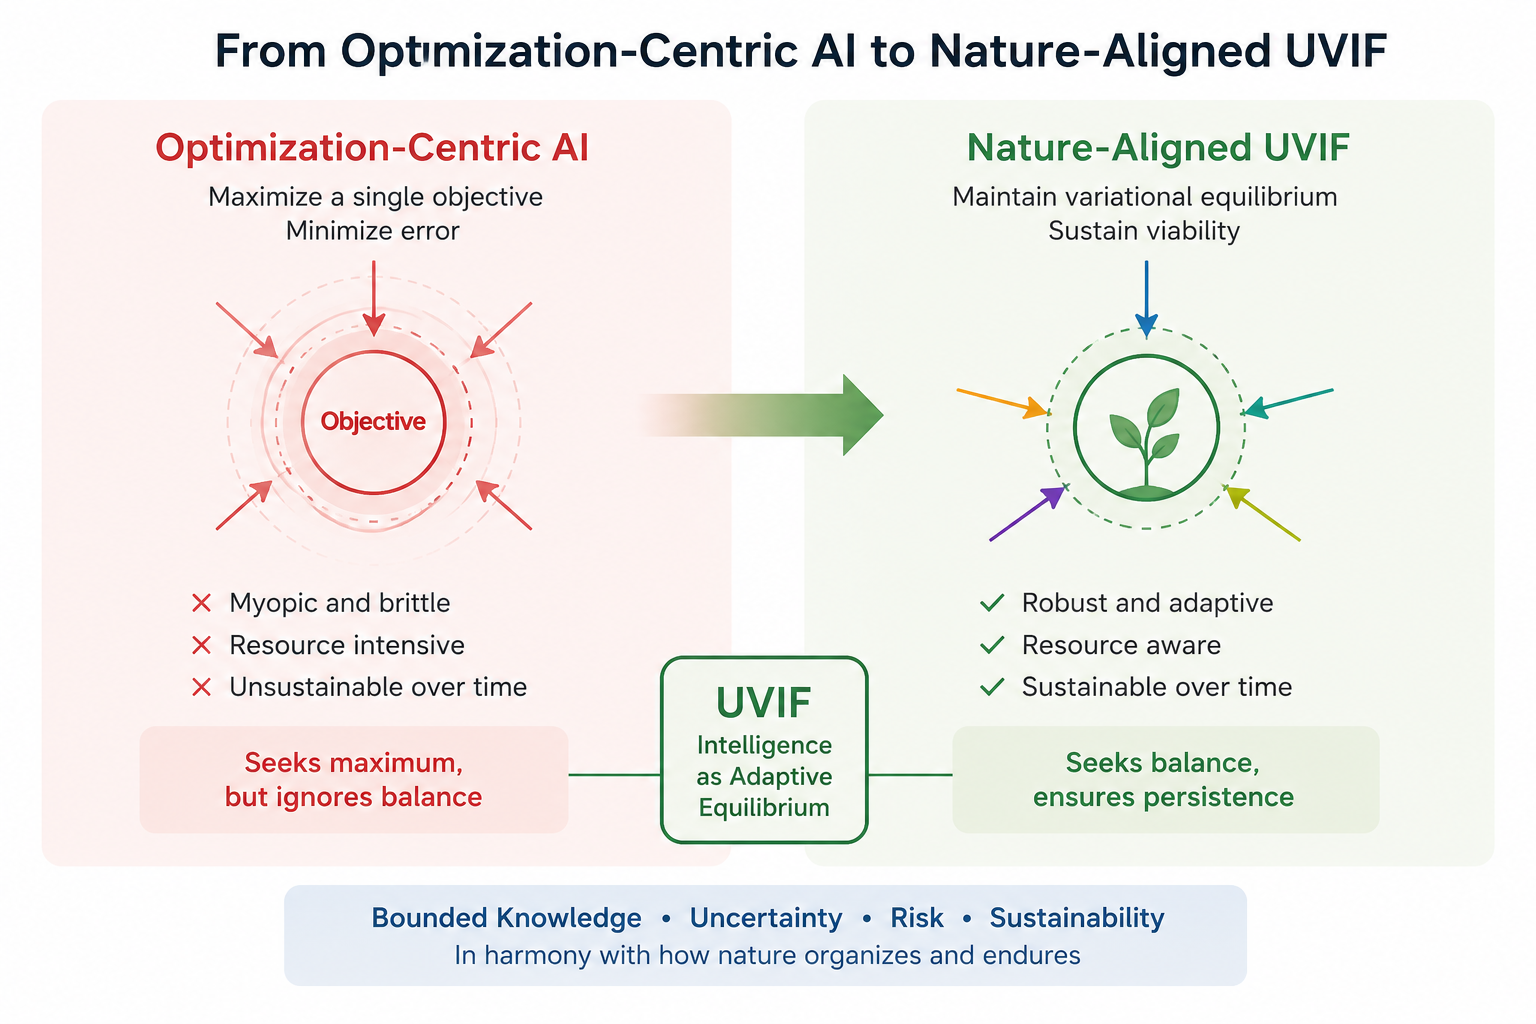
\includegraphics[width=\linewidth]{Figures/Fig1_UVIF_Motivation.png}
\caption{From optimization-centric artificial intelligence toward
nature-aligned variational equilibrium. Conventional optimization-driven
AI typically focuses on maximizing a single objective or minimizing a
single error function. In contrast, UVIF interprets intelligence as the
maintenance of adaptive equilibrium under bounded knowledge,
uncertainty, resource constraints, risk, and long-term sustainability.
Rather than pursuing isolated maximization, the framework seeks
persistent viability and balanced adaptation across competing
organizational forces.}
\label{fig:uvif_motivation}
\end{figure}

Fig.~\ref{fig:uvif_motivation} illustrates the conceptual transition
proposed in this work. On the left side, conventional optimization-based
AI is represented as a system attempting to maximize a single objective
through increasingly aggressive minimization of error. While such
systems may achieve strong short-term performance, they often become
fragile, resource-intensive, and difficult to sustain under changing
real-world conditions.

The right side of the figure introduces the central intuition of
\uvif{}. Instead of seeking absolute maximization, intelligent systems
are viewed as adaptive entities operating under multiple competing
pressures. These pressures include uncertainty, limited resources,
bounded observability, temporal constraints, and the need for long-term
stability. Under this perspective, intelligence is not defined by
perfect certainty or exhaustive optimization, but by the ability to
maintain coherent and sustainable operation despite incomplete
knowledge and environmental variability.

The transition arrow shown in the figure symbolically represents the
shift from optimization-oriented intelligence toward equilibrium-oriented
intelligence. The plant at the center of the UVIF side emphasizes that
persistent natural systems rarely survive through isolated maximization.
Instead, nature tends to preserve viable adaptive balance across
changing conditions. UVIF adopts this organizational principle as a
foundation for sustainable intelligent-system design.

\subsection{Main Contributions}

This paper makes the following contributions to the study of
intelligence:

\begin{enumerate}[label=(\arabic*)]
  \item \textbf{A formal conceptual architecture.} We introduce the five
    core forces of \uvif{}---epistemic pull, selective protection,
    computational drag, action efficiency, and sustainability---together
    with the admissibility constraints that bound their joint operation,
    and we derive the concept of Variational Equilibrium as their
    natural stable point.

  \item \textbf{Philosophical and scientific foundations.} We ground
    \uvif{} in variational principles from physics, homeostasis from
    physiology, self-organization from ecology, and the free-energy
    principle from neuroscience \citep{friston2010fep,bettinger2023physiological},
    constructing a coherent interdisciplinary narrative.

  \item \textbf{A positioning within cognitive systems research.} We
    contrast \uvif{} with the frameworks nearest to it in this
    field---predictive processing and active inference, resource-rational
    analysis, allostatic regulation, and integrated cognitive
    architectures---identifying in each case what the framework shares,
    what it omits, and what it adds, and stating the trade-offs honestly
    rather than claiming uniform advantage.

  \item \textbf{Cross-domain illustrations.} We demonstrate how
    \uvif{} applies to biological regulation, ecological resilience,
    human cognition, artificial autonomous systems, and organizational
    management, sketching case studies in healthcare, smart energy,
    autonomous transport, cybersecurity, and long-term organizational
    intelligence.

  \item \textbf{Discriminating predictions and a research agenda.} We
    state, as hypotheses rather than results, the empirical predictions
    that would separate \uvif{} from competing accounts, and articulate
    the open mathematical, empirical, and engineering work required to
    test them.
\end{enumerate}

We are explicit about what this paper does not do. It develops a
conceptual architecture and the predictions it generates; it reports no
empirical experiments, and none of its claims are presented as
established results. The accompanying simulation exercises the
framework's own dynamics and is not offered as evidence about cognitive
systems in operation. The five forces are posited on the strength of
their recurrence across independently developed literatures, not
derived; the Variational Equilibrium manifold is defined but its
existence and stability conditions are not proved. These gaps are
stated as such in Section~\ref{sec:limitations} rather than deferred
to a concluding caveat.

The remainder of the paper proceeds as follows. Section~\ref{sec:optimization_equilibrium}
diagnoses the limitations of the dominant optimization paradigm.
Section~\ref{sec:foundations} constructs the philosophical and scientific
foundations of \uvif{}.
Section~\ref{sec:uvif_framework} presents the full framework architecture.
Section~\ref{sec:applications_nature} surveys applications across natural
and artificial systems.
Section~\ref{sec:cognitive_systems} develops the cognitive case in
detail and positions the framework against predictive processing,
resource-rational analysis, allostasis, and cognitive architectures.
Section~\ref{sec:case_studies} develops concrete case studies.
Section~\ref{sec:comparative} positions \uvif{} relative to existing frameworks.
Section~\ref{sec:implications} draws theoretical implications.
Section~\ref{sec:limitations} acknowledges limitations and open challenges.
Section~\ref{sec:future} outlines future research directions.
Section~\ref{sec:conclusion} concludes.



% =========================
% Deep philosophical revision inserted
% =========================

\subsection{Bounded Knowability and the Limits of Exhaustive Certainty}

A foundational assumption underlying the UVIF philosophy is that intelligent systems embedded within reality cannot obtain complete simultaneous knowledge of all relevant variables governing their environment and future evolution. This limitation is not merely technological or computational; rather, it reflects a deeper structural condition associated with bounded observability and irreducible uncertainty \citep{lieder2019resourcerational,clark2013whatever}.

Modern optimization-driven artificial intelligence frequently operates under the implicit assumption that increasing data, computational power, and model complexity will asymptotically reduce uncertainty and eventually approach near-complete predictive certainty. UVIF challenges this assumption. Natural systems rarely operate under exhaustive certainty. Biological organisms, ecological systems, and human cognition continuously make adaptive decisions under incomplete, evolving, and partially hidden information \citep{lieder2019resourcerational,schulkin2019allostasis}.

Principles such as quantum uncertainty illustrate a broader epistemological insight: reality itself may impose structural limits on complete simultaneous disclosure of all relevant variables. UVIF does not invoke quantum mechanics as a direct computational mechanism for intelligence, but rather as an illustration that bounded knowability may be a fundamental condition of embedded systems interacting with reality \citep{fankhauser2025epistemic,busch2007heisenberg}.

Consequently, intelligent action cannot indefinitely wait for maximal knowledge. Delayed action itself carries risk, cost, and potential loss of viability. Sustainable intelligence therefore emerges not from perfect prediction, but from the capacity to maintain adaptive equilibrium under incomplete information, temporal pressure, and constrained resources \citep{callaway2022rational,schulkin2019allostasis}.
